\begin{block}{Finite Size Analysis of Entanglement Spectra}
\begin{columns}[T]
\begin{column}{.5\textwidth}
        \begin{figure}[hbctp]
        \centering
        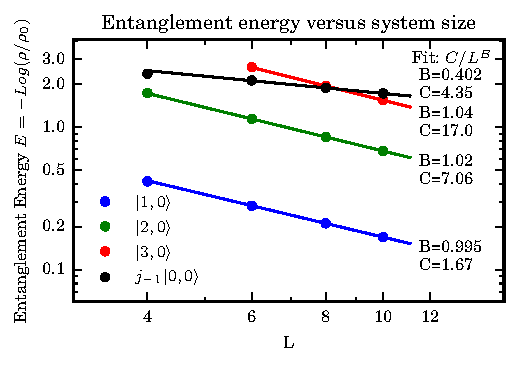
\includegraphics{{interpolatedboson/a10/plots/EntanglementEnergyScaling2.pdf}}
        %\caption{Power law fits for the lowest three states above the ground state at momentum zero and lowest two states at momentum 1 in Figure \ref{fig:sc-EEFinitesize}. The $1/L$ scaling is a signature of a gapless (entanglement) Hamiltonian. The labeling of the states $\ket{e, m}$ or $j_{-1} \ket{e, m}$ is explained in the CFT section below.}
        %\label{fig:sc-EEScaling}
        \end{figure}
        \bi 
        \item<1-> Low energy modes show gapless $1/L$ behavior
        \ei
\end{column}
\begin{column}{.5\textwidth}
\begin{figure}[hbctp]
\centering
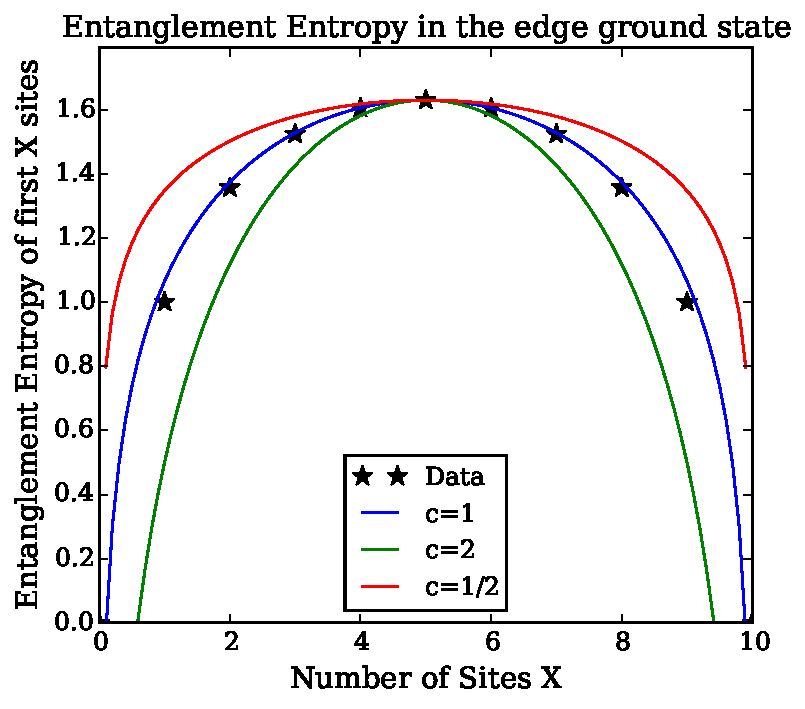
\includegraphics{{interpolatedboson/a0/plots/edge_gs_EE.pdf}}
%\caption{Entanglement entropy within the entanglement ground state of the soft-core boson state on $10$ sites. For comparison, the Cardy-Calabrese formula $S(x) = c/3 \log \sin( \pi x/L) + const.$ is shown with $c=\frac{1}{2}, 1,$ and $2$, with the $const.$ fixed by matching the maximum of the entanglement entropy data. $c=1$ is a good fit.}
%\label{fig:hc-edge-gs-ee}
\end{figure}
\bi
\item Fix this to show topological entanglement entropy is 0
\ei
\end{column}
\end{columns}


\end{block}